\documentclass[fontsize=12pt,a4paper]{article}

% for margins
\usepackage{geometry}
\geometry{
	top = 20mm,
	headsep = 6mm,
	left = 22mm,
	right = 22mm, 
	bottom = 26mm,
}

% to insert images
\usepackage{graphicx}
\usepackage{array}
\usepackage{wrapfig}

% for date format
\usepackage[yyyymmdd]{datetime} 
\renewcommand{\dateseparator}{.}

% for tables
\usepackage{tabularx} 

%  for hyperlinks
\usepackage{hyperref}

% for better paragraphs
\usepackage{parskip}

% for bra-ket notation
\usepackage{braket}

% for figure
\usepackage[magyar]{babel} % Magyar nyelvi támogatás
\renewcommand{\figurename}{\arabic{figure}. ábra}

% --------------
% The documennt
% --------------

\begin{document}

% loading the authors
\newcommand{\authorI}{Bánáti Benedek}
\newcommand{\neptunI}{123456}
\newcommand{\authorII}{Horváth Kristóf}
\newcommand{\neptunII}{123456}
\newcommand{\authorIII}{Tóth Balázs Gábor}
\newcommand{\neptunIII}{123456}
\newcommand{\authorIV}{Tóth Bálint}
\newcommand{\neptunIV}{123456}

% the actual title page
\begin{titlepage}
\begin{center}


\includegraphics[width=0.6\textwidth]{bme_logo_kicsi.jpg}
\vspace{2.5cm}

{\huge Bloch-gömb szimulátor előzetes leadás}
\vspace{0.75cm}

\textsc{\Large Kvantuminformatikai alkalmazások}

{\today}
\vspace{2cm}

% for full width table use this instead: 
%\begin{tabularx}{\textwidth}{X r}

\begin{tabular}{l r}
 \authorI \hspace{2cm} & \neptunI \\ 
 \authorII  & \neptunII \\  
 \authorIII & \neptunIII \\
 \authorIV  & \neptunIV
\end{tabular}


\vspace{2cm}


\tableofcontents

\end{center}
\end{titlepage}

% The main content
\newpage
\section{Más Bloch-gömb szimulátorok}

% Qiskit
\vspace{0.4cm}
\subsection{Qiskit}
\textbf{Forrás: \href{https://www.ibm.com/quantum/qiskit}{ibm.com/quantum/qiskit}} 

\begin{wrapfigure}{r}{0.38\textwidth}
    \vspace{-0.6cm} % to remove padding
    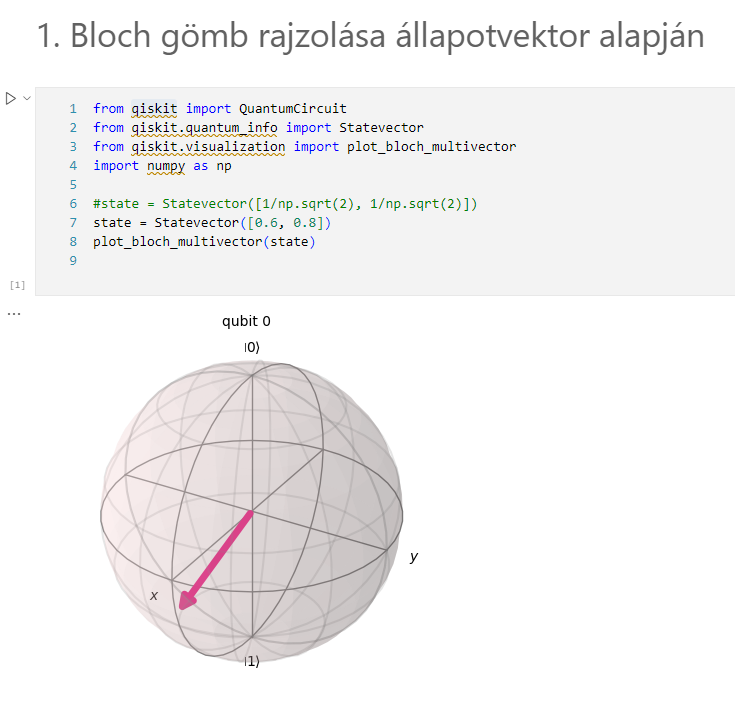
\includegraphics[width=0.9\linewidth]{Simulators/Qiskit.png} 
\end{wrapfigure}

Jupyter környezetben a gyakorlat során ismerkedtünk meg az IBM eszközével. Nem kifejezetten Bloch-gömb szimulátornak tervezték, de sok funkcióval rendelkezik, amik ezt a használati módot is lehetővé teszik.

Előny:

\begin{itemize}
    \item A kapuk helyesen működnek, könnyen paraméterezhetők.
    \item Bármilyen állapotú Qubit-et használhatunk.
    \item Könnyen átlátható.
    \item Szimulációk is futtathatók.
    \item Komplikáltabb feladatokra is használható.
\end{itemize}

Hátrány:

\begin{itemize}
    \item A környezetet telepíteni kell.
    \item Nem valósidőben látjuk a változást.
    \item A kapuk hatása nehezebben követhető.
    \item Több állapot megjelenítésére külön gömböket használ.
\end{itemize}


% Bits and electrons
\vspace{0.4cm}
\subsection{Bits And Electrons}
\textbf{Forrás: \href{https://bits-and-electrons.github.io/bloch-sphere-simulator/}{bits-and-electrons.github.io/bloch-sphere-simulator/}}

Egy webes bloch gömb szimulátor, amely a kapuk bemutatására fókuszál.

Előny:

\begin{itemize}
    \item A kapuk hatását animációval mutatja.
    \item Valósidőben láthatjuk az állapotot.
    \item Saját kapuk létrehozása vektor és forgatási szög megadásával.
    \item Előre definiált kapuk: X,Y,Z,H.
    \item Előre definiált fél/negyed/nyolcad fordulat kapuk.
    \item Lambda kapuk: X és Y tengely körül pontos szöggel forgatás.
\end{itemize}

Hátrány:

\begin{itemize}
    \item Csak 1 qubit ábrázolása.
    \item Nem írható be a kiinduló állapot a felhasználói felületen keresztül.
    \item Csak kapuk segítségével lehet módosítani az állapotot.
    \item Hiába animálja a kapukat, az utukat nem rajzolja be, sok kapunál nehezebben lekövethető.
    \item Nehezen állítható alaphelyzetbe. Ki kell törölni a linkből a tulajdonságokat.
    \item Néha eltűnnek bizonyos grafikai elemek.
\end{itemize}

% Bloch kerp
\vspace{0.4cm}
\subsection{Bloch Kerb}
\textbf{Forrás: \href{https://bloch.kherb.io/}{bloch.kherb.io}}

Egy webes bloch gömb vizualizáló, amely főleg a forgatásokra fokuszál.

Előny:

\begin{itemize}
    \item Vizualizálja a műveletek útját így könnyebben elképzelhető.
    \item Saját kapuk létrehozása forgatási szögek megadásával.
    \item Forgatási tengely és a régebbi lépések színei is állíthatók.
    \item Állítható, hogy hány hamarabbi lépést mutasson.
    \item Vissza lehet vonni a korábban megtett léptetéseket.
    \item Könnyen alaphelyzetbe állítható.
\end{itemize}

Hátrány:

\begin{itemize}
    \item Csak 1 qubit ábrázolása.
    \item Nem írhatóak be az egyes állapotok UI-n keresztül.
    \item Csak előre definiált kapuk használhatók.
    \item Minden változtatás után visszaállítja az alapértelmezett nézetre.
    \item Nem mutatja valós időben a hozzá tartozó értékeket.
    \item Nem lehet megadni a qubit kiinduló állapotát.
\end{itemize}


% Attila Kun
\vspace{0.4cm}
\subsection{Attila Kun}
\textbf{Forrás: \href{https://attilakun.net/bloch/}{attilakun.net/bloch}}

Egy webes bloch gömb vizualizáló, amely főleg az átlátható, logikus, kényelmes nézetre fokuszál.

Előny:

\begin{itemize}
    \item Vizualizálja a műveletek útját így könnyebben elképzelhető.
    \item Könnyen alaphelyzetbe állítható.
    \item Állítható a kiinduló állapot.
    \item Beállítható azonnal a négy alapértelmezett bázis állapot.
    \item A kiinduló állapot állítható a kurzor segítségével vagy pontos adatokat megadni az UI-n keresztül lehet.
    \item Mátrix megadásával lehet saját kaput létrehozni.
    \item Előre definiált kapuk: X,Y,Z,H
\end{itemize}

Hátrány:

\begin{itemize}
    \item Csak 1 qubit ábrázolása.
    \item Az irányítás nem teljesen egyértelmű.
    \item Nem lehet több kaput alkalmazni.
    \item Nem jelenik meg a gömb.
\end{itemize}

\vspace{0.4cm}
\subsection{Quantum 3D visualizer}
\textbf{Forrás: \href{https://apps.microsoft.com/detail/9pj77hf1w39t?ocid=webpdpshare}{Microsoft Store Link}}

Előny:

\begin{itemize}
    \item Állítható a kiinduló állapot.
    \item Valósidőben láthatjuk az állapotot.
    \item User Interface-n keresztül állíthatóak a kapuk, theta és phi szögek.
    \item Kapuk egybecsatolása.
    \item Animált lépés.
    \item Sok előre definiált kapu.
    \item Kurzorral lehet állítani az állapotot.
\end{itemize}

\noindent Hátrány:

\begin{itemize}
    \item Csak 1 qubit ábrázolására képes.
    \item Nem rajzolja be az útvonalat.
\end{itemize}

% Spec
\newpage
\section{Szoftverkövetelmény specifikáció}

\subsection{Cél}
A szoftver fő célja, hogy könnyen átláthatóan, felhasználó barát módon vizualizálja a Bloch gömböt, ahol könnyen állíthatjuk a kapukat és a qubiteket. Továbbá az is fontos szempont volt, hogy több mint 1 qubitet tudjon ábrázolni a programunk.

\subsection{Részletes feladatok}
A programban könnyedén lehessen qubiteket hozzáadni, módosítani a kiinduló állapotaikat. Legyen öt különböző beépített kapu típus: X, Y, Z, Hadamard és Phase. Az adott qubithez lehessen új kaput rögzíteni, a sorrenden változtatni, törölni, egybecsatolni és a Phase kapuk paramétereit változtatni. Egy kiválasztott kapunál egérrel tudjuk megnézni egy kis lebegő ablakban a mátrixát.

A változtatások legyenek berajzolv, és lehessen állítani a qubit és a hozzátartozó (kapuk hatására létrejövő) útvonal  színét. Ennek az útvonalnak az elrejtésére is legyen lehetősége a felhasználóknak programon belül. A színválasztásnál az alfa csatorna is legyen állítható, hogy a többi állapotot jobban láthassuk. 

A program folyamatosan jelenítse meg a gömb körül a $\ket{0}$ és $\ket{1}$ bázisállapotokat.

A qubitek értékadásánál arra is biztosítson a program lehetőséget, hogy használjuk az sqrt függvényt, azaz egy szám pontos gyökértékét használja a számításoknál, ahogyan ez az alább lévő képen is látszódik.

A gömböt a kurzor segítségével lehet forgatni, hogy más szögből is megtekinthessük a qubitek állapotait.

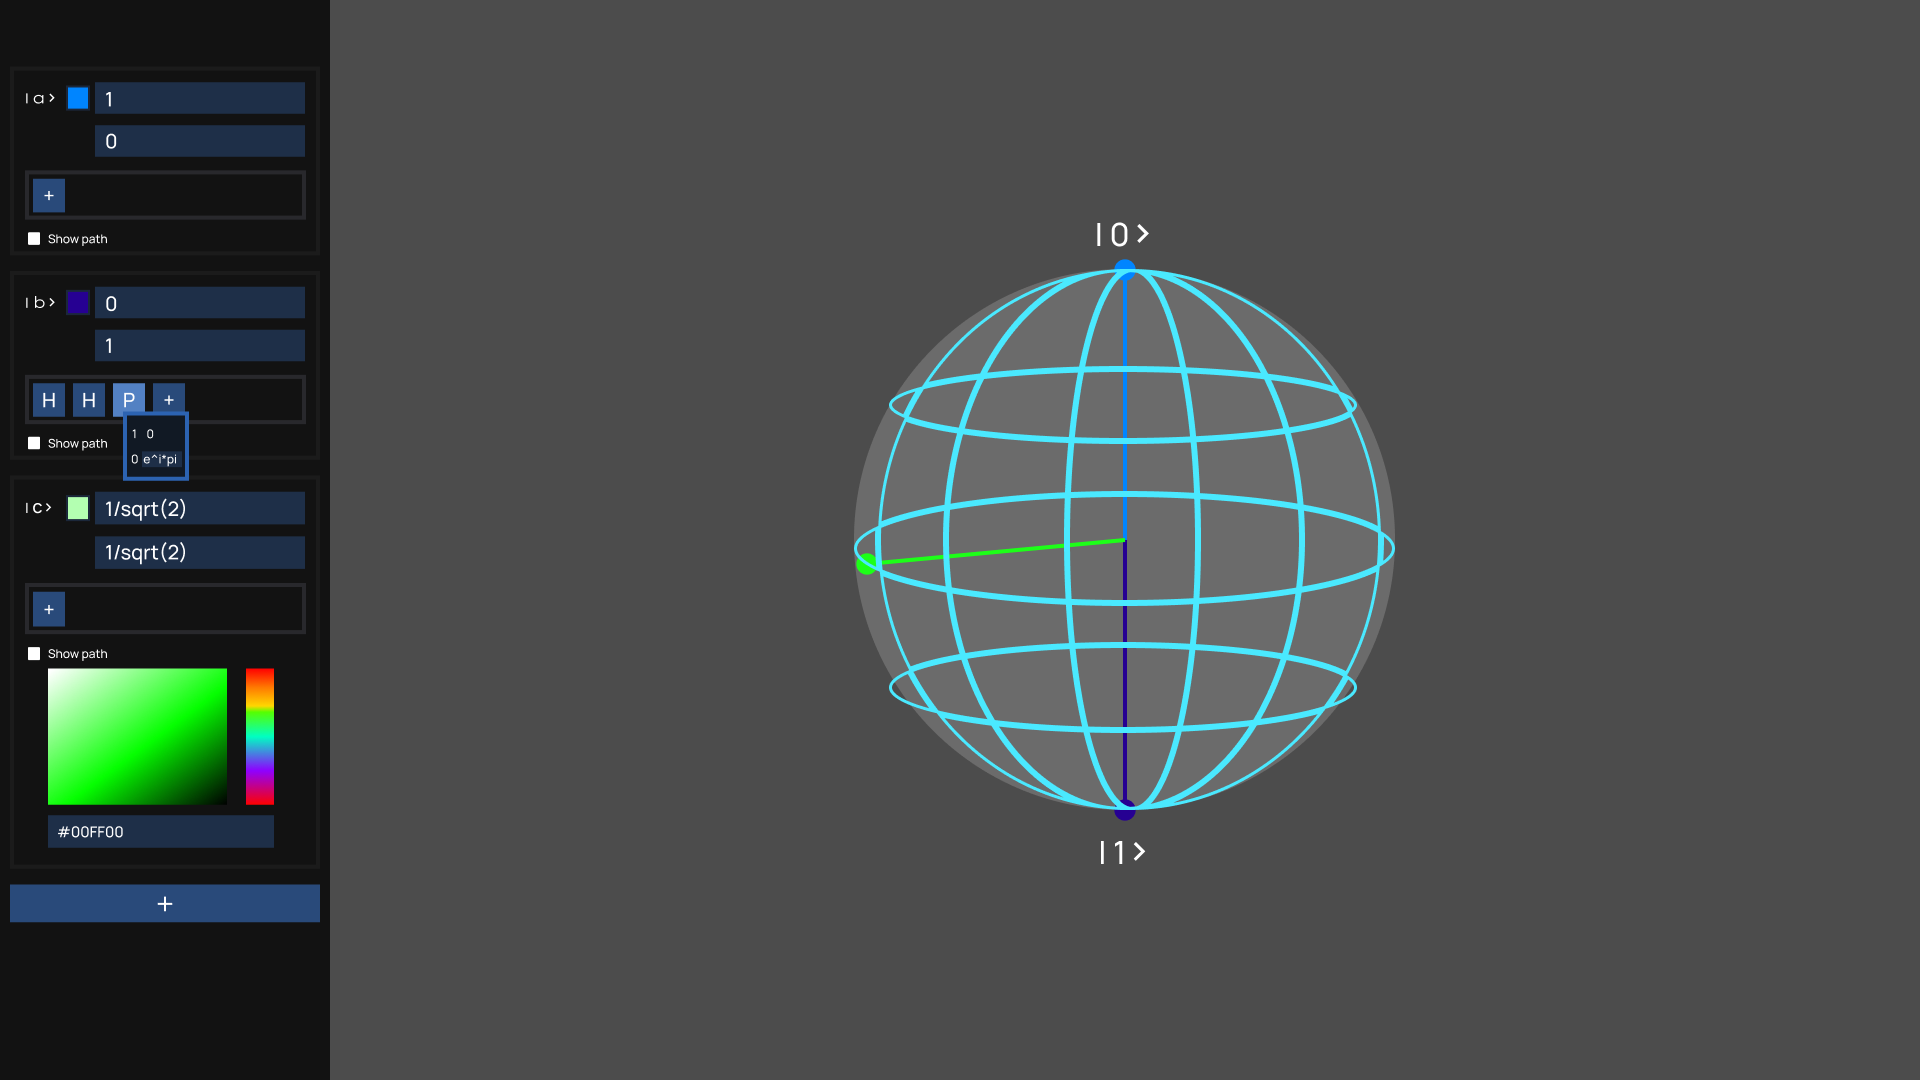
\includegraphics[width=1.0\textwidth]{Bloch-sphere.png}
\href{https://www.figma.com/design/X1JXQDatg8IsLa6VYQFRTJ/Bloch-sphere}{Figma design link}

% Fejlesztői környezet
\newpage
\section{Fejlesztőkörnyezet megnevezése}

\begin{itemize}
    \item \textbf{Godot:}  Godot game engine mellett döntöttünk, mivel könnyen használható, könnyűvé teszi a pluginok használatát és nyílt forráskodú. A saját programozási nyelvében, a \href{https://docs.godotengine.org/en/stable/tutorials/scripting/gdscript/gdscript_basics.html}{gdscript}-ben már sok funkció implementálva van, ami segít nekünk a program elkészítésében. Ebben a környezetben tervezzük leprogramozni a megjelenítéshez szükséges logikát és shadereket.
    \item \textbf{ImGui for Godot:} a godot beépített UI rendszerét nem találtuk alkalmasnak a feladatra, ezért hosszas keresés után az \href{https://godotengine.org/asset-library/asset/2985}{ImGui} mellett döntöttünk. Ezzel a könyvtárral lehetséges megvalósítani a kapuk cserélgetését, a színválasztót, a pop-up ablakok megjelenítését és a saját bemeneti mezők alkalmazását.
    \item \textbf{Egyéb fejlesztéshez használt eszközök:} Visual Studio Code, Git, GitHub, Overleaf
\end{itemize}

\newpage
\section{Felhasználói dokumentáció}

A felhasználói dokumentáció fő feladata, hogy bemutassa az alkalmazás használatát. A témával kapcsolatos ismereteket igényel, az elmélet nincs benne elmagyarázva.

\subsection{Telepítés}
Az alábbi github repository-ban (\href{https://github.com/RandomByteFF/bloch-sphere-simulator/releases/}{link}) elérhető program. A verziók közül választhatunk, érdemes a legújabbat választani. Verzión belül 4 lehetőség közül választhatunk. A program letöltéséhez a windows/linux.zip fájlt válasszuk, az operációs rendszertől függően. A zip fájlt kicsomagolva a program futtatható.

\subsection{Alapértelmezett állapot}
A program betöltése után az alábbi képpel találkozunk.

\begin{figure}[h]
    \centering
    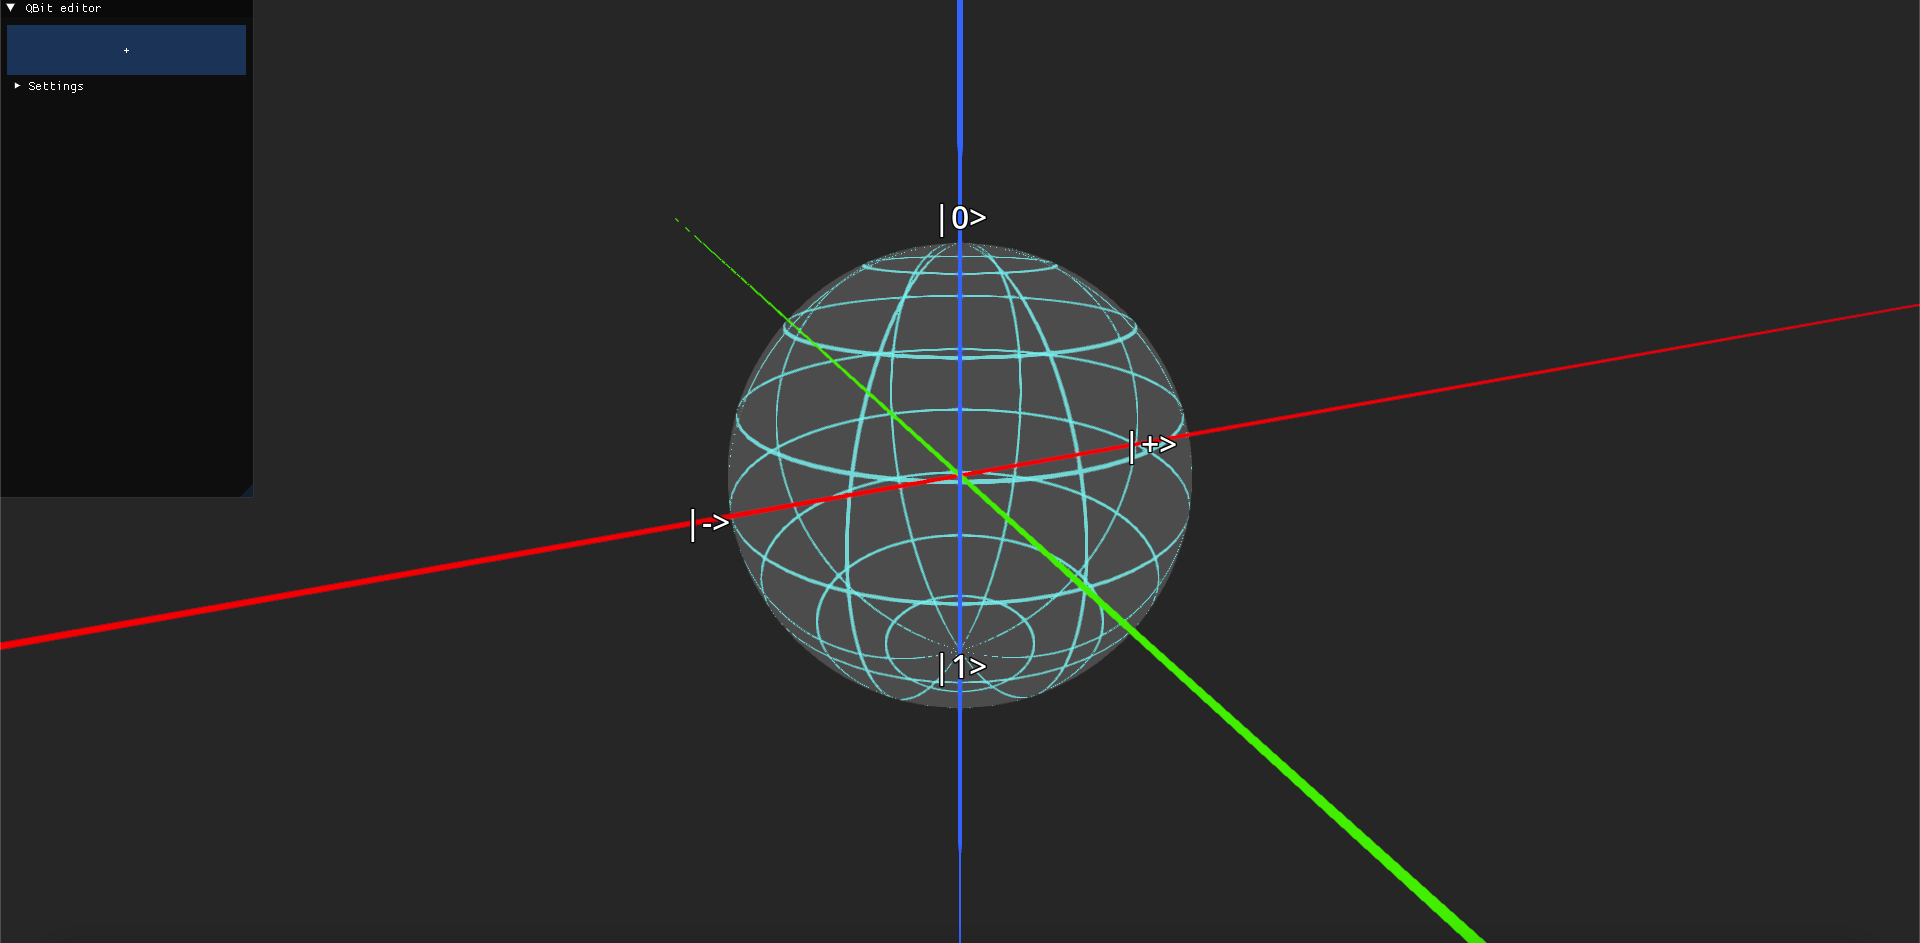
\includegraphics[width=1.0\linewidth]{App/default.png} 
    \caption{Betöltés utáni állapot}
\end{figure}

Az alaphelyzetet mutató képen több minden látható. Először a Bloch-gömb vizualizációja, mely alapértelmezetten nem tartalmaz qubitet. A képernyő bal oldalán a \textbf{Qubit kezelőfelület} helyezkedik el. Látható a színes koordináta rendszer, ahol az x tengely színe piros, y tengely színe kék, z tengely színe zöld. 4 fontos állapot is jelölve van a gömbön: $\ket{0}, \ket{1}, \ket{+}, \ket{-}$. 

\newpage
\subsection{Qubit kezelés}
A széles '+' feliratú gombra kattintva vehetünk fel egy új qubitet. Ezután a \textbf{Qubit kezelőfelületen} megjelenik $\ket{+}$ alapértelmezett értékekkel. Továbbá látható, hogy nem tartozik hozzá kapu. 

A qubitet tudjuk törölni is a DEL gomb segítségével.

\begin{figure}[h]
    \centering
    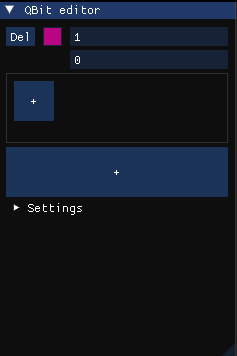
\includegraphics[height=7.2cm]{App/add_qubit.png}
    \caption{\textbf{Qubit kezelőfelület}}
\end{figure}

\subsection{Kapuk kezelése}
A qubithez tartozik egy kisebb plusz gomb. Erre kattintva megjelenik a kapu választó felület az programban támogatott összes lehetséges kapuval. A kapuk egymás után vannak fűzve, alkalmazásuk balról jobbra történik. 
Sorrendjük megcserélhető, a bal egér gomb kattintással és lenyomva tartásával arrébb húzhatjuk a kaput a kívánt helyre. 
Ezen felül lehet törölni is kapukat. Ezt úgy tudja megtenni a felhasználó, hogy bal egér gombbal kattint egy kapura, melynek következtében megjelenik egy gomb, amin a "Delete gate" szöveg olvasható. Ezt megnyomva törlődik a kapu. Az \textbf{U} kapunál megjelenik a hozzátartozó mátrix, mely értékeit természetesen át lehet írni a komplex szám algebrai formájában. A \textbf{P} kapunál pedig a fázisért felelős paramétert állíthatjuk

Kapuk:
\begin{itemize}
    \item X: Pauli-X
    \item Y: Pauli-Y
    \item Z: Pauli-Z
    \item H: Hadamard
    \item P: Phase
    \item I: Identity/Egység
    \item U: Unitér mátrix
\end{itemize}

\begin{figure}[h]
    \centering
    \begin{minipage}{0.3\linewidth}
        \raggedright
        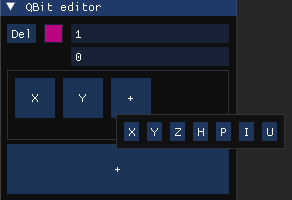
\includegraphics[width=\linewidth]{App/qubit_gates.png}
        \caption{Kapu hozzáadása}
    \end{minipage}%
    \hfill
    \begin{minipage}{0.3\linewidth}
        \centering
        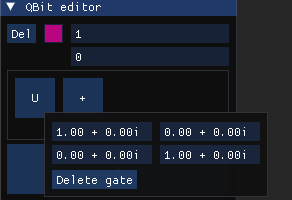
\includegraphics[width=\linewidth]{App/unitary.png}
        \caption{Unitér mátrix}
    \end{minipage}%
    \hfill
    \begin{minipage}{0.3\linewidth}
        \raggedleft
        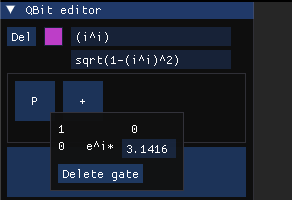
\includegraphics[width=\linewidth]{App/phase.png}
        \caption{Phase kapu állító felülete}
    \end{minipage}
\end{figure}

\newpage
\subsection{Szín állítás}
A \textbf{Qubit kezelőfelület}en DEL gomb mellett látható egy szín gomb, melyre a kurzort helyezve megjelenik egy információs ablak, melyben a szín adatai vannak leírva. A gombra kattintva megjelenik alatta a \textbf{színválasztó felület}. Látható a RGBA és HSVA színtartomány, melynek értékeit úgy lehet szerkeszteni, hogy dupla kattintunk a szerkeszteni kivánt attribútumra és beírjuk az új értékét. Továbbá lehet \textit{hexadecimális} értéket megadni. A hozzátartozó szövegdobozba elég egyszer bele kattintani, hogy tudjuk szerkeszteni. Ezek megváltoztatják a qubithez tartozó nyilat és az utat.

\begin{figure}[h]
    \centering
    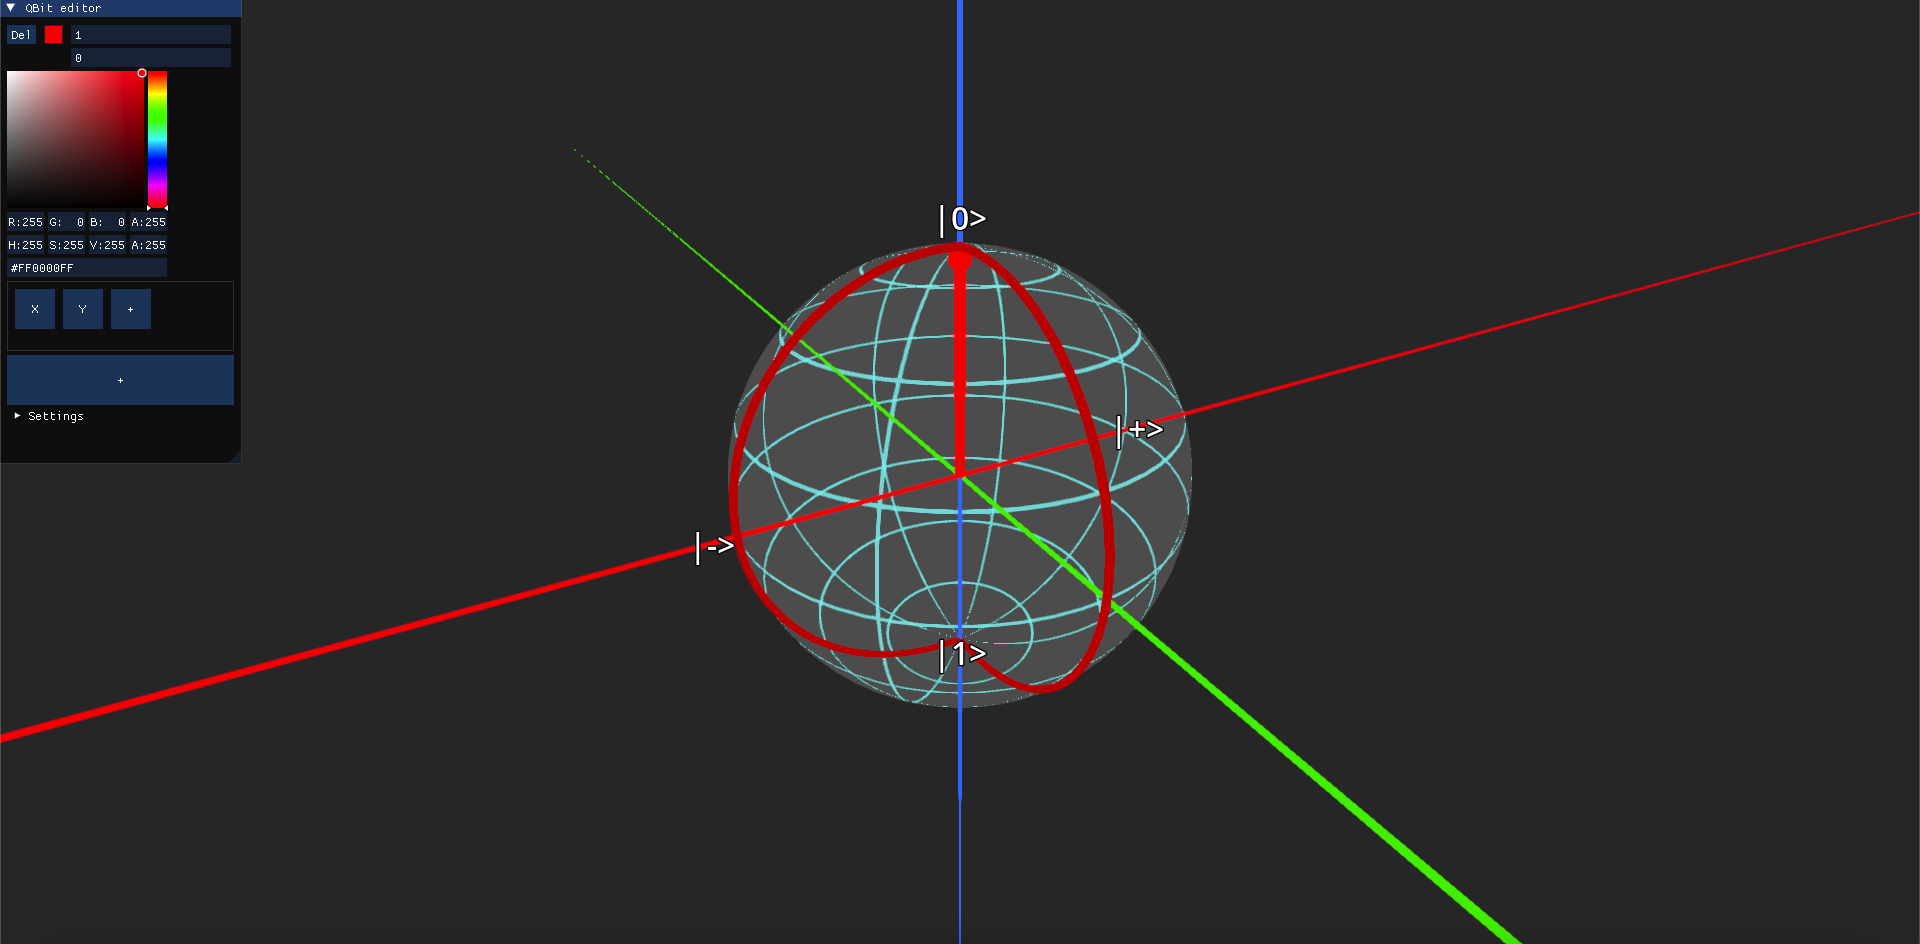
\includegraphics[width=1.0\linewidth]{App/color.png}
    \caption{Szín állítás eredménye}
\end{figure}

A színválasztó felület bezárásához ismét a színt tartalmazó gombra kell kattintani. Mivel ez a gomb követi a színek változását, ezért a színek segítenek a qubitek beazonosításában akkor is, ha a válaszó rész el van rejtve.


\newpage
\subsection{Kifejezés értelmező}
A \textbf{Qubit kezelőfelület}en a qubit értékéhez nemcsak valós számok írhatók, hanem komplex számú kifejezések is. A qubit értékénél a szöveg beviteli mezőbe a karakter limit 80, azaz a program 79 karaktert enged beírni. Az unitér mátrix értékmezőinél pedig 32, azaz 31-et engedélyez a szoftver.

Példák a kifejezés használatra: i\^{}i vagy sqrt(1-(i\^{}i)\^{}2).

A program nem tesz különbséget a kis és nagybetűk között. Például: SIN(PI) = sin(pi)
\begin{table}[h!]
    \centering
    \resizebox{0.7\textwidth}{!}{ % Táblázat méretezése a teljes szélesség 70%-ára
    \begin{tabular}{|c|c|c|}
        \hline
        \textbf{Operáció} & \textbf{Szimbólum} & \textbf{Példa} \\ \hline
        Összeadás        & +                  &  8 + pi        \\ \hline
        Kivonás          & -                  &  8 - pi        \\ \hline
        Szorzás          & *                  &  8 * pi        \\ \hline
        Osztás           & /                  &  8 / pi        \\ \hline
        Hatványra emelés & \^{}               &  8 \^{} pi     \\ \hline
        Sin              & sin                &  sin(pi)       \\ \hline
        Cos              & cos                &  cos(pi)       \\ \hline
        Tan              & tan                &  tan(pi)       \\ \hline
        Négyzetgyök      & sqrt               &  sqrt(4761)    \\ \hline
        Pi               & pi                 &  8 * pi        \\ \hline
        Euler-szám       & e                  &  e \^{} 8      \\ \hline
        Képzetes egység  & i                  &  8 * i         \\ \hline
    \end{tabular}
    }
    \caption{Matematikai operációk és szimbólumok}
\end{table}

\begin{figure}[h]
    \centering
    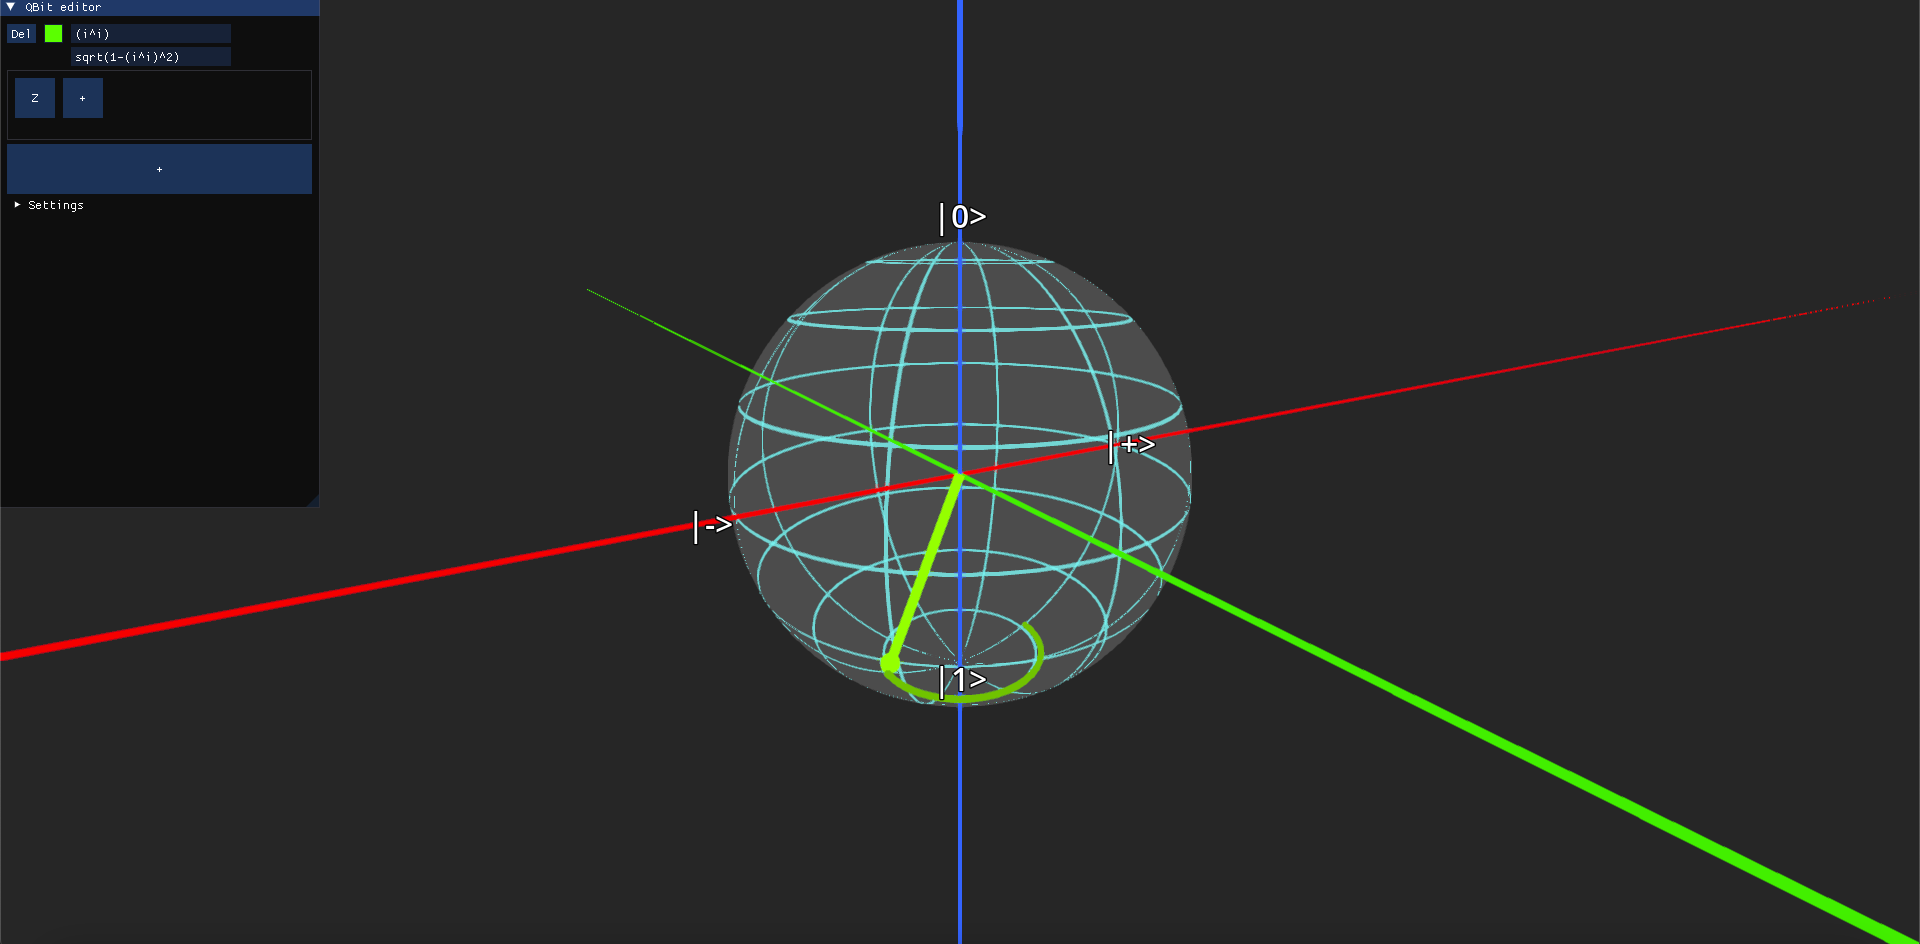
\includegraphics[width=1.0\linewidth]{App/expression.png}
    \caption{Kifejezés példa}
\end{figure}

\newpage
\subsection{Több qubit vizualizálása}
A program fő része, hogy korlátlan qubitet tud megjeleníteni. Amennyiben nem fér el a \textbf{Qubit kezelőfelület}en az összes qubit, akkor megjelenik egy görgetősáv, és úgy lehet navigálni köztük. El lehet rejteni a qubitet is azzal, hogy átlátszóvá teszzük. Ezt legegyszerűbben úgy lehet elérni, hogy a hexadecimálisan megadott színkód végére 2 db 0-t kell beírni.

\begin{figure}[h]
    \centering
    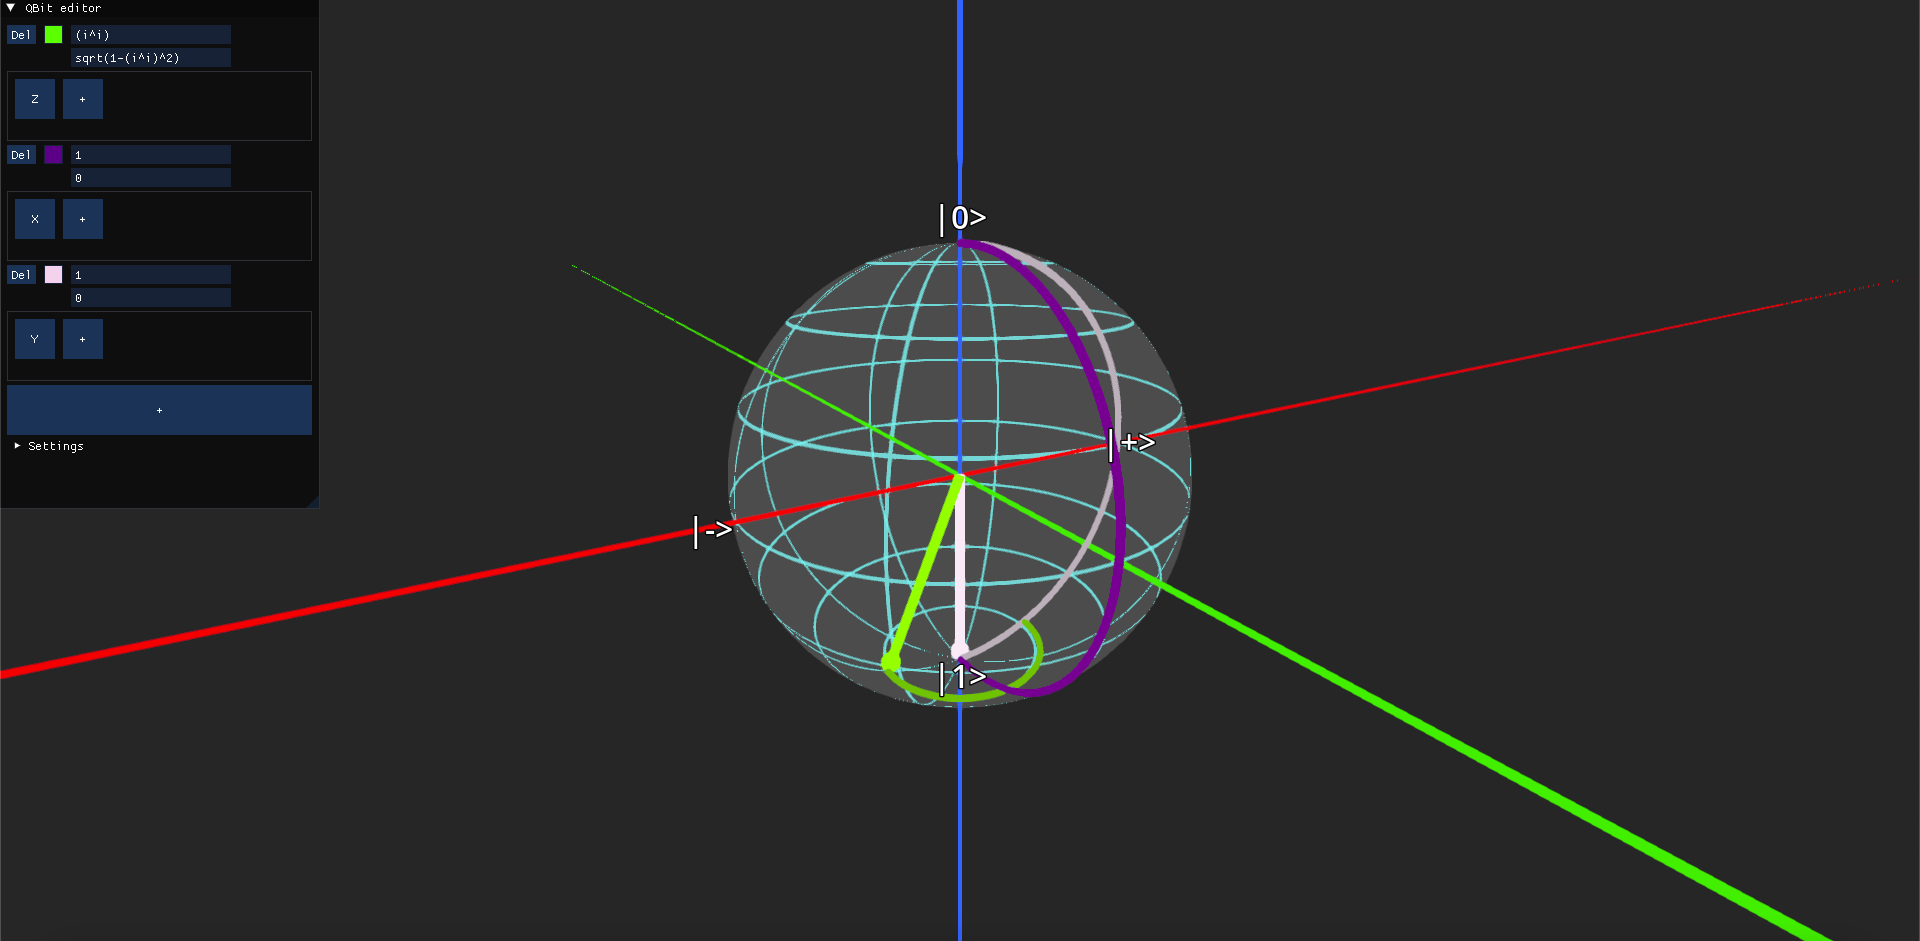
\includegraphics[width=1.0\linewidth]{App/nqubit.png}
    \caption{Több qubit ábrázolása}
\end{figure}

\subsection{Beállítás}
A \textbf{Qubit kezelőfület}en található egy \textit{Settings} fül. Itt három beállítást tudunk állítani. Igaz/hamis típusok, azaz ha be van pipálva a beállítás, akkor igaz lesz, ha nincs akkor hamis.

\begin{table}[h]
    \centering
    \vspace{-\arrayrulewidth} % Eltünteti a sortörés helyét a két rész között
    \resizebox{0.7\textwidth}{!}{\begin{tabular}{|c|c|} % Tartalom
        \hline
        \textbf{Beállítás} & \textbf{Leírás} \\ \hline
        Show axis & Tengely mutatása \\ \hline
        Show ket labels & $\ket{a}$ szövegek mutatása a gömbön \\ \hline
        Show grid lines 3.1 & Rács vonalak mutatása a gömb felületén \\ \hline
    \end{tabular}}
\end{table}

\begin{figure}[h]
    \centering
    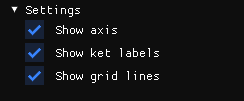
\includegraphics[width=0.4\linewidth]{App/settings.png}
    \caption{Beállítás felület}
\end{figure}

\subsection{További navigáció a felületen}
\begin{itemize}
\item Bal egér gombbal való kattintás után lenyomva tartva tudjuk forgatni a gömböt. Továbbá görgővel lehet ki/be közelíteni. Fel görgetéssel közelebbről, le görgetéssel pedig távolabbról tekinthetjük meg a gömböt. 
\item A \textbf{Qubit kezelőfelület} átméretezhető. A jobb alsó sarkát kell megfogni bal egér gomb lenyomásával és az egér mozgatás hatására változik a mérete. 
\item A programot a jobb felül található X gombbal lehet bezárhni. Ilyenkor az állapot nem kerül mentésre, így a következő használatnál ismét az 1. ábrán látható állapot fog megjelenni.
\end{itemize}

\newpage
\section{Programozói dokumentáció}

A programozói dokumentáció csak egy általános leírást ad a forráskódról. A belső működés nincs kifejtve. %kristóf majd fogalmazd át buta vagyok

\subsection{Kifejezés kezelő}
Ebben az alfejezetben a \textbf{Kifejezés kezelő}höz tartozó osztályok leírása van. Rövid leírás arról, hogy hogyan lett megvalósítva a program ezen része.

\subsubsection{ExpressionHandler}
Az ExpressionHandler osztály kifejezések kiértékelésére szolgál. Ez az osztály lehetővé teszi a felhasználók számára, hogy matematikai kifejezéseket adjanak meg, melyeket komplex számmá alakít.

\begin{table}[h]
    \centering
    \resizebox{1.0\textwidth}{!}{%
    \begin{tabular}{|m{6cm}|p{10cm}|} % Az első oszlop m{...}, a második p{...}
        \hline
        \textbf{Metódus} & \textbf{Leírás} \\ \hline
        evaluate(text: String) -$>$ Complex & Kiértékeli a megadott szöveget és visszaadja az eredményt komplex számként. \\ \hline
    \end{tabular}}
\end{table}

\subsubsection{Token}
A Token egy olyan adatstruktúra, amely a bemeneti karakterlánc egyes részeit reprezentálja, például számokat, operátorokat, zárójeleket és függvényeket. A tokenek segítenek a bemeneti kifejezés szintaktikai értelmezésében.

\begin{table}[h]
    \centering
    \resizebox{1.0\textwidth}{!}{%
    \begin{tabular}{|m{6cm}|p{10cm}|} % Az első oszlop m{...}, a második p{...}
        \hline
        \textbf{Attribútum} & \textbf{Leírás} \\ \hline
        type & A token típusa (érték, operátor, zárójel, függvény). \\ \hline
        value & A token értéke. \\ \hline
        precedence & Meghatározza a műveleti sorrendet. \\ \hline
    \end{tabular}}
\end{table}

\subsubsection{Tokenizer}
A Tokenizer osztály a megadott szöveget tokenekre bontja, amelyeket később a parser feldolgozhat.

\begin{table}[h!]
    \centering
    \resizebox{1.0\textwidth}{!}{%
    \begin{tabular}{|m{6cm}|p{10cm}|} % Az első oszlop m{...}, a második p{...}
        \hline
        \textbf{Attribútum} & \textbf{Leírás} \\ \hline
        brackets & A zárójelek listája. \\ \hline
        operators & Az operátorok és azok precedenciája. \\ \hline
        functions & Az értelmezett függvények listája. \\ \hline
        values & Az értelmezett értékek listája. \\ \hline
    \end{tabular}}
\end{table}

\begin{table}[h!]
    \centering
    \resizebox{1.0\textwidth}{!}{%
    \begin{tabular}{|m{6cm}|p{10cm}|} % Az első oszlop m{...}, a második p{...}
        \hline
        \textbf{Metódus} & \textbf{Leírás} \\ \hline
        tokenize(text: String) -$>$ Array[Token] & A kapott szöveget tokenekre bontja és visszaadja azok listáját. \\ \hline
        insert\_multiplication(tokens: \newline  Array[Token]) -$>$ Array[Token] & Beszúrja a szorzás operátort a megfelelő helyekre a tokenek között, ha szükséges. Pl.: 3pi = 3 * pi \\ \hline
    \end{tabular}}
\end{table}

\subsubsection{Parser}
A Parser osztály egy módosított shunting yard algoritmust használ. Ez az osztály a tokenekből kifejezésfát épít, amelyet később ki lehet értékelni.

\begin{table}[h!]
    \centering
    \resizebox{1.0\textwidth}{!}{%
    \begin{tabular}{|m{6cm}|p{10cm}|} % Az első oszlop m{...}, a második p{...}
        \hline
        \textbf{Metódus} & \textbf{Leírás} \\ \hline
        parse(tokens: Array[Token]) -$>$ \newline Array[ExpressionNode] & Kiértékeli a kapott tokeneket és visszaadja normál lengyel jelöléssel a szükségeseket. \\ \hline
    \end{tabular}}
\end{table}

\newpage

\subsubsection{ExpressionNode}
Az ExpressionNode osztály a kifejezésfában lévő csomópontokat reprezentálja. Minden csomópont egy tokent, valamint bal és jobb gyerek csomópontokat tartalmazhat.

\begin{table}[h!]
    \centering
    \resizebox{1.0\textwidth}{!}{
    \begin{tabular}{|m{6cm}|p{10cm}|} % Az első oszlop m{...}, a második p{...}
        \hline
        \textbf{Attribútum} & \textbf{Leírás} \\ \hline
        token & A csomópontot reprezentáló token. \\ \hline
        left & A bal oldali gyerek csomópont. \\ \hline
        right & A jobb oldali gyerek csomópont. \\ \hline
        takes & A csomópont által igényelt operandusok száma. \\ \hline
        \_backup\_value & A csomópont által a hiányzó értékek helyére behelyettesített érték. (Pl. -2 = 0-2) \\ \hline
        \_operation & A csomópont által végrehajtott művelet. \\ \hline
    \end{tabular}}
\end{table}

\subsection{GUI}

Ebben az alfejezetben a \textbf{grafikus felhasználói felület}et megvalósító osztályok leírása található.

\subsubsection{Gui}

A Gui osztály a fő \textbf{grafikus felhasználói felület}et (GUI) kezeli. Ez az osztály kezeli a különböző GUI elemeket, mint például a tengelyeket, címkéket, a \textbf{Qubit kezelőfelület}et és a gömb objektumot.

\subsubsection{QubitGui}

A QubitGui osztály feladata a kvantumbitek (qubit) grafikus felhasználói felületének kezelése és megjelenítése. Ez az osztály felelős a kvantumbitekhez kapcsolódó beállítások, például a színek és kapuk kezeléséért és megjelenítéséért az ImGui könyvtáron keresztül.

\begin{table}[h]
    \centering
    \resizebox{\textwidth}{!}{%
    \begin{tabular}{|m{6cm}|p{10cm}|}
        \hline
        \textbf{Attribútum} & \textbf{Leírás} \\ \hline
        text1 & Az első szövegmező tartalma. \\ \hline
        text2 & A második szövegmező tartalma. \\ \hline
        color & A qubit színe. \\ \hline
        gates & A qubithez tartozó kapuk grafikus felületének listája (ezek tárolják a kapukat is). \\ \hline
    \end{tabular}}
\end{table}

\begin{table}[h!]
    \centering
    \resizebox{\textwidth}{!}{%
    \begin{tabular}{|m{6cm}|p{10cm}|}
        \hline
        \textbf{Metódus} & \textbf{Leírás} \\ \hline
        gui() & Újra rendereli a kvantumbithez tartozó felhasználói felületet. \\ \hline
    \end{tabular}}
\end{table}

\subsubsection{GateGui}

A GateGui osztály egy kvantumkapu \textbf{grafikus felhasználói felület}ének (GUI) kezelésére szolgál. Ez az osztály lehetővé teszi a felhasználók számára, hogy megjelenítsék és módosítsák a kvantumkapu paramétereit.

\begin{table}[h!]
    \centering
    \resizebox{\textwidth}{!}{%
    \begin{tabular}{|m{6cm}|p{10cm}|}
        \hline
        \textbf{Attribútum} & \textbf{Leírás} \\ \hline
        gate & A kvantumkapu objektum. \\ \hline
    \end{tabular}}
\end{table}

\begin{table}[h!]
    \centering
    \resizebox{\textwidth}{!}{%
    \begin{tabular}{|m{6cm}|p{10cm}|}
        \hline
        \textbf{Metódus} & \textbf{Leírás} \\ \hline
        gui(clickable: bool = true) & Rendereli a kapu GUI-t. A kattinthatóságot paraméterként kapja, ez vezérli, hogy a felugró ablak megjelenhet-e. \\ \hline
    \end{tabular}}
\end{table}

\newpage
\subsubsection{CustomGateGui}

A CustomGateGui osztály egy egyedi kvantumkapu grafikus felhasználói felületének (GUI) kezelésére szolgál. Ez az osztály lehetővé teszi a felhasználók számára, hogy megadják és módosítsák a kapu mátrixának elemeit. Az osztály tartalmaz egy felugró ablakot, amelyben a felhasználók beállíthatják a kapu paramétereit.

\begin{table}[h!]
    \centering
    \resizebox{\textwidth}{!}{%
    \begin{tabular}{|m{6cm}|p{10cm}|}
        \hline
        \textbf{Attribútum} & \textbf{Leírás} \\ \hline
        a, b, c, d & A kapu mátrixának elemei. \\ \hline
    \end{tabular}}
\end{table}

\subsubsection{PhaseGateGui}

A PhaseGateGui osztály egy GateGui osztályból származtatott GUI-komponens, amely egy kvantumkapu grafikus kezelőfelületének megvalósítására szolgál. Kifejezetten egy fáziskapu (Phase Gate) interakciójához készült, és lehetővé teszi a felhasználó számára a kapuhoz tartozó paraméterek megtekintését és módosítását.

\begin{table}[h!]
    \centering
    \resizebox{\textwidth}{!}{%
    \begin{tabular}{|m{6cm}|p{10cm}|}
        \hline
        \textbf{Művelet} & \textbf{Leírás} \\ \hline
        update\_gate() & Frissíti a kapu aktuális állapotát. \\ \hline
    \end{tabular}}
\end{table}

\subsection{MathData}

Ebben az alfejezetben a komplex számok, mátrixok és vektorok kezelésére szolgáló osztályok bemutatásáról van szó.

\subsubsection{Complex}

A Complex osztály komplex számok kezelésére szolgál. Ez az osztály lehetővé teszi a komplex számok különböző matematikai műveleteinek elvégzését, mint például az összeadás, kivonás, szorzás és osztás.

\begin{table}[h]
    \centering
    \resizebox{\textwidth}{!}{%
    \begin{tabular}{|m{6cm}|p{10cm}|}
        \hline
        \textbf{Attribútum} & \textbf{Leírás} \\ \hline
        re & A valós rész. \\ \hline
        im & A képzetes rész. \\ \hline
    \end{tabular}}
\end{table}

\begin{table}[h!]
    \centering
    \begin{tabular}{|p{6cm}|p{10cm}|}
        \hline
        \textbf{Metódus} & \textbf{Függvény neve} \\ \hline
        Konjugált & conjugate \\ \hline
        Összeadás & add \\ \hline
        Kivonás & subtract \\ \hline
        Szorzás & multiply \\ \hline
        Szorzás valós számmal & multiply\_real \\ \hline
        Polar formából létrehozás & new\_polar \\ \hline
    \end{tabular}
\end{table}

\newpage
\subsubsection{MatrixComplex2D}

A MatrixComplex2D osztály 2D komplex mátrixok kezelésére szolgál. Ez az osztály lehetővé teszi a mátrixok különböző matematikai műveleteinek elvégzését, mint például az összeadás, szorzás és transzponálás. A mátrix sorfolytonos mátrix, e-szerint kell megadni az a,b,c,d értékeket.

\begin{table}[h!]
    \centering
    \resizebox{\textwidth}{!}{%
    \begin{tabular}{|m{6cm}|p{10cm}|}
        \hline
        \textbf{Attribútum} & \textbf{Leírás} \\ \hline
        a & A mátrix első eleme. \\ \hline
        b & A mátrix második eleme. \\ \hline
        c & A mátrix harmadik eleme. \\ \hline
        d & A mátrix negyedik eleme. \\ \hline
    \end{tabular}}
\end{table}

\begin{table}[h!]
    \centering
    \begin{tabular}{|p{6cm}|p{10cm}|}
        \hline
        \textbf{Művelet} & \textbf{Függvény neve} \\ \hline
        Összeadás & add \\ \hline
        Vektor szorzás & multiply\_vec \\ \hline
        Mátrix szorzás & multiply\_mat \\ \hline
        Skalár szorzás & multiply\_scalar \\ \hline
        Transzponálás & transpose \\ \hline
        Adjungált képzés & adjugate \\ \hline
    \end{tabular}
\end{table}

\subsubsection{VectorComplex2D}

A VectorComplex2D osztály 2D komplex vektorok kezelésére szolgál. Ez az osztály lehetővé teszi a vektorok különböző matematikai műveleteinek elvégzését, mint például az összeadás és szorzás.

\begin{table}[h!]
    \centering
    \resizebox{\textwidth}{!}{%
    \begin{tabular}{|m{6cm}|p{10cm}|}
        \hline
        \textbf{Attribútum} & \textbf{Leírás} \\ \hline
        x & A vektor első eleme. \\ \hline
        y & A vektor második eleme. \\ \hline
    \end{tabular}}
\end{table}

\begin{table}[h!]
    \centering
    \begin{tabular}{|p{6cm}|p{10cm}|}
        \hline
        \textbf{Művelet} & \textbf{Függvény neve} \\ \hline
        Összeadás & add \\ \hline
        Vektor szorzás & multiply\_vec \\ \hline
        Mátrix szorzás & multiply\_mat \\ \hline
        Normalizálás & normalize \\ \hline
        Skalár szorzás & multiply\_scalar \\ \hline
    \end{tabular}
\end{table}

\newpage
\subsection{További osztályok}

Azon osztályok leírása mely nem lett bekategorizálva.

\subsubsection{QubitControl}

A QubitControl osztály egy kvantumbit (qubit) vezérlésére szolgál. Ez az osztály kezeli a qubit állapotát, a hozzá tartozó nyilat és a kapukat. Az osztály különböző eseményekre reagál, mint például a kapuk hozzáadása, átrendezése vagy eltávolítása, valamint a qubit állapotának változása. Az osztály tartalmazza a qubit állapotának vizualizációjához szükséges interpolációs görbét és útvonalat is.

\begin{table}[h!]
    \centering
    \resizebox{\textwidth}{!}{%
    \begin{tabular}{|m{6cm}|p{10cm}|}
        \hline
        \textbf{Attribútum} & \textbf{Leírás} \\ \hline
        arrow & A nyíl, amely a qubit állapotát jelzi. \\ \hline
        qubit & A qubit állapota. \\ \hline
        gates & A qubithez tartozó kapuk listája. \\ \hline
        interpolation & Egy 3D görbe, amely az interpolációs pontokat tartalmazza. \\ \hline
        path & Az útvonal, amelyet a qubit követ. \\ \hline
    \end{tabular}}
\end{table}

\subsubsection{ControlStore}

A ControlStore egy singleton osztály, ami a qubit vezérlők tárolására szolgál. Ez az osztály egy listában tárolja a QubitControl objektumokat, és lehetőséget biztosít új qubit vezérlők hozzáadására. Az osztály célja, hogy központi helyet biztosítson a qubit vezérlők kezelésére és nyilvántartására.

\begin{table}[h]
    \centering
    \resizebox{\textwidth}{!}{%
    \begin{tabular}{|m{6cm}|p{10cm}|}
        \hline
        \textbf{Metódus} & \textbf{Leírás} \\ \hline
        add\_qubit(data) & Hozzáad egy új qubit vezérlőt a tárolóhoz. \\ \hline
    \end{tabular}}
\end{table}

\subsubsection{PathDrawn}

A PathDrawn osztály egy 3D útvonal rajzolására szolgál. Ez az osztály kezeli az útvonal görbéjét és annak vizualizációját. Az osztály lehetőséget biztosít az útvonal színének és sugárának beállítására, valamint az útvonal pontjainak frissítésére.

\begin{table}[h!]
    \centering
    \resizebox{\textwidth}{!}{%
    \begin{tabular}{|m{6cm}|p{10cm}|}
        \hline
        \textbf{Attribútum} & \textbf{Leírás} \\ \hline
        line\_radius & Az útvonal vonalának sugara. \\ \hline
        res & A kirajzoláshoz használt henger közelítésének felbontása. \\ \hline
    \end{tabular}}
\end{table}

\begin{table}[h!]
    \centering
    \resizebox{\textwidth}{!}{%
    \begin{tabular}{|m{6cm}|p{10cm}|}
        \hline
        \textbf{Metódus} & \textbf{Leírás} \\ \hline
        set\_path(curve: Curve3D) & Beállítja a görbét, amely kirajzolásra kerül. \\ \hline
        set\_color(color: Array, percentage: float) & Beállítja a kirajzolás színét. \\ \hline
    \end{tabular}}
\end{table}

\subsubsection{Arrow}

Az Arrow osztály egy 3D nyíl kezelésére szolgál, amely a qubit állapotát jelzi a Bloch-gömbön. Az osztály lehetővé teszi a nyíl irányának és színének beállítását.

\begin{table}[h!]
    \centering
    \resizebox{\textwidth}{!}{%
    \begin{tabular}{|m{6cm}|p{10cm}|}
        \hline
        \textbf{Attribútum} & \textbf{Leírás} \\ \hline
        model & A nyíl 3D modellje. \\ \hline
    \end{tabular}}
\end{table}

\begin{table}[h!]
    \centering
    \resizebox{\textwidth}{!}{%
    \begin{tabular}{|m{6cm}|p{10cm}|}
        \hline
        \textbf{Metódus} & \textbf{Leírás} \\ \hline
        set\_point(point: Vector3) & Beállítja a nyíl irányát a megadott pont felé. \\ \hline
        set\_color(color: Array) & Beállítja a nyíl színét. \\ \hline
    \end{tabular}}
\end{table}

\newpage
\subsubsection{Camera3D}

A Camera3D osztály egy 3D kamera kezelésére szolgál. Az osztály lehetővé teszi a kamera érzékenységének, zoom érzékenységének és zoom távolságának beállítását, valamint a célpont és a forgáspont meghatározását.

\begin{table}[h!]
    \centering
    \resizebox{\textwidth}{!}{%
    \begin{tabular}{|m{6cm}|p{10cm}|}
        \hline
        \textbf{Attribútum} & \textbf{Leírás} \\ \hline
        sensitivity & A kamera érzékenysége. \\ \hline
        zoom\_sensitivity & A zoom érzékenysége. \\ \hline
        max\_zoom\_distance & A maximális zoom távolság. \\ \hline
        min\_zoom\_distance & A minimális zoom távolság. \\ \hline
        pivot & A kamera forgáspontja. \\ \hline
    \end{tabular}}
\end{table}

\subsubsection{Gate}

A Gate osztály egy kvantumkapu kezelésére szolgál. Ez az osztály lehetővé teszi a kvantumkapuk különböző típusainak és azok mátrixainak kezelését.

\begin{table}[h!]
    \centering
    \resizebox{\textwidth}{!}{%
    \begin{tabular}{|m{6cm}|p{10cm}|}
        \hline
        \textbf{Attribútum} & \textbf{Leírás} \\ \hline
        name & A kapu neve. \\ \hline
        abbreviation & A kapu rövidítése. \\ \hline
        value & A kapu mátrix reprezentációja. \\ \hline
        cache & A kapu által létrehozott módosítást eltároló cache. \\ \hline
        sphere\_radius & A Bloch-gömb sugara. \\ \hline
    \end{tabular}}
\end{table}

\subsubsection{Qubit}

A Qubit osztály egy kvantumbit (qubit) kezelésére szolgál. Ez az osztály lehetővé teszi a qubit állapotának és annak különböző műveleteinek kezelését.

\begin{table}[h!]
    \centering
    \resizebox{\textwidth}{!}{%
    \begin{tabular}{|m{6cm}|p{10cm}|}
        \hline
        \textbf{Metódus} & \textbf{Leírás} \\ \hline
        from\_vec(val: VectorComplex2D) $\rightarrow$ Qubit & Létrehoz egy qubitet egy vektorból. \\ \hline
        is\_valid() $\rightarrow$ bool & Ellenőrzi, hogy a qubit állapota érvényes-e. \\ \hline
        to\_bloch\_sphere\_pos(use\_godot\_coords: bool) $\rightarrow$ Vector3 & Visszaadja a qubit 3D reprezentációját a Bloch-gömbön. \\ \hline
    \end{tabular}}
\end{table}

\end{document}